\documentclass[aspectratio=169,10pt]{beamer}
\usetheme{Madrid}
\usecolortheme{default}
\usepackage{graphicx}
\usepackage{booktabs}

\title[Polar Sea-Ice Timing]{Polar Sea-Ice Timing:\\Classical Trends and a Rigorous Spatial Null Test}
\subtitle{University of Hamburg --- 6-credit Sea Ice Course (June/July 2026)}
\author{Omkar Kondhalkar}
\date{}

\begin{document}

\begin{frame}
  \titlepage
\end{frame}

\begin{frame}{Core finding (locked)}
  \textbf{Magnitude loss $\neq$ calendar shift.}
  \begin{itemize}
    \item Arctic min DOY: $-0.08$~d~yr$^{-1}$, $p = 0.65$ (not significant)
    \item Antarctic AFIN: $+29.45$~d~yr$^{-1}$, $p = 0.21$ (not significant)
    \item Phase~2 asks: does \emph{spatial} pre-melt ice state explain the noise?
  \end{itemize}
\end{frame}

\begin{frame}{Phase 1: No significant timing shift}
  \centering
  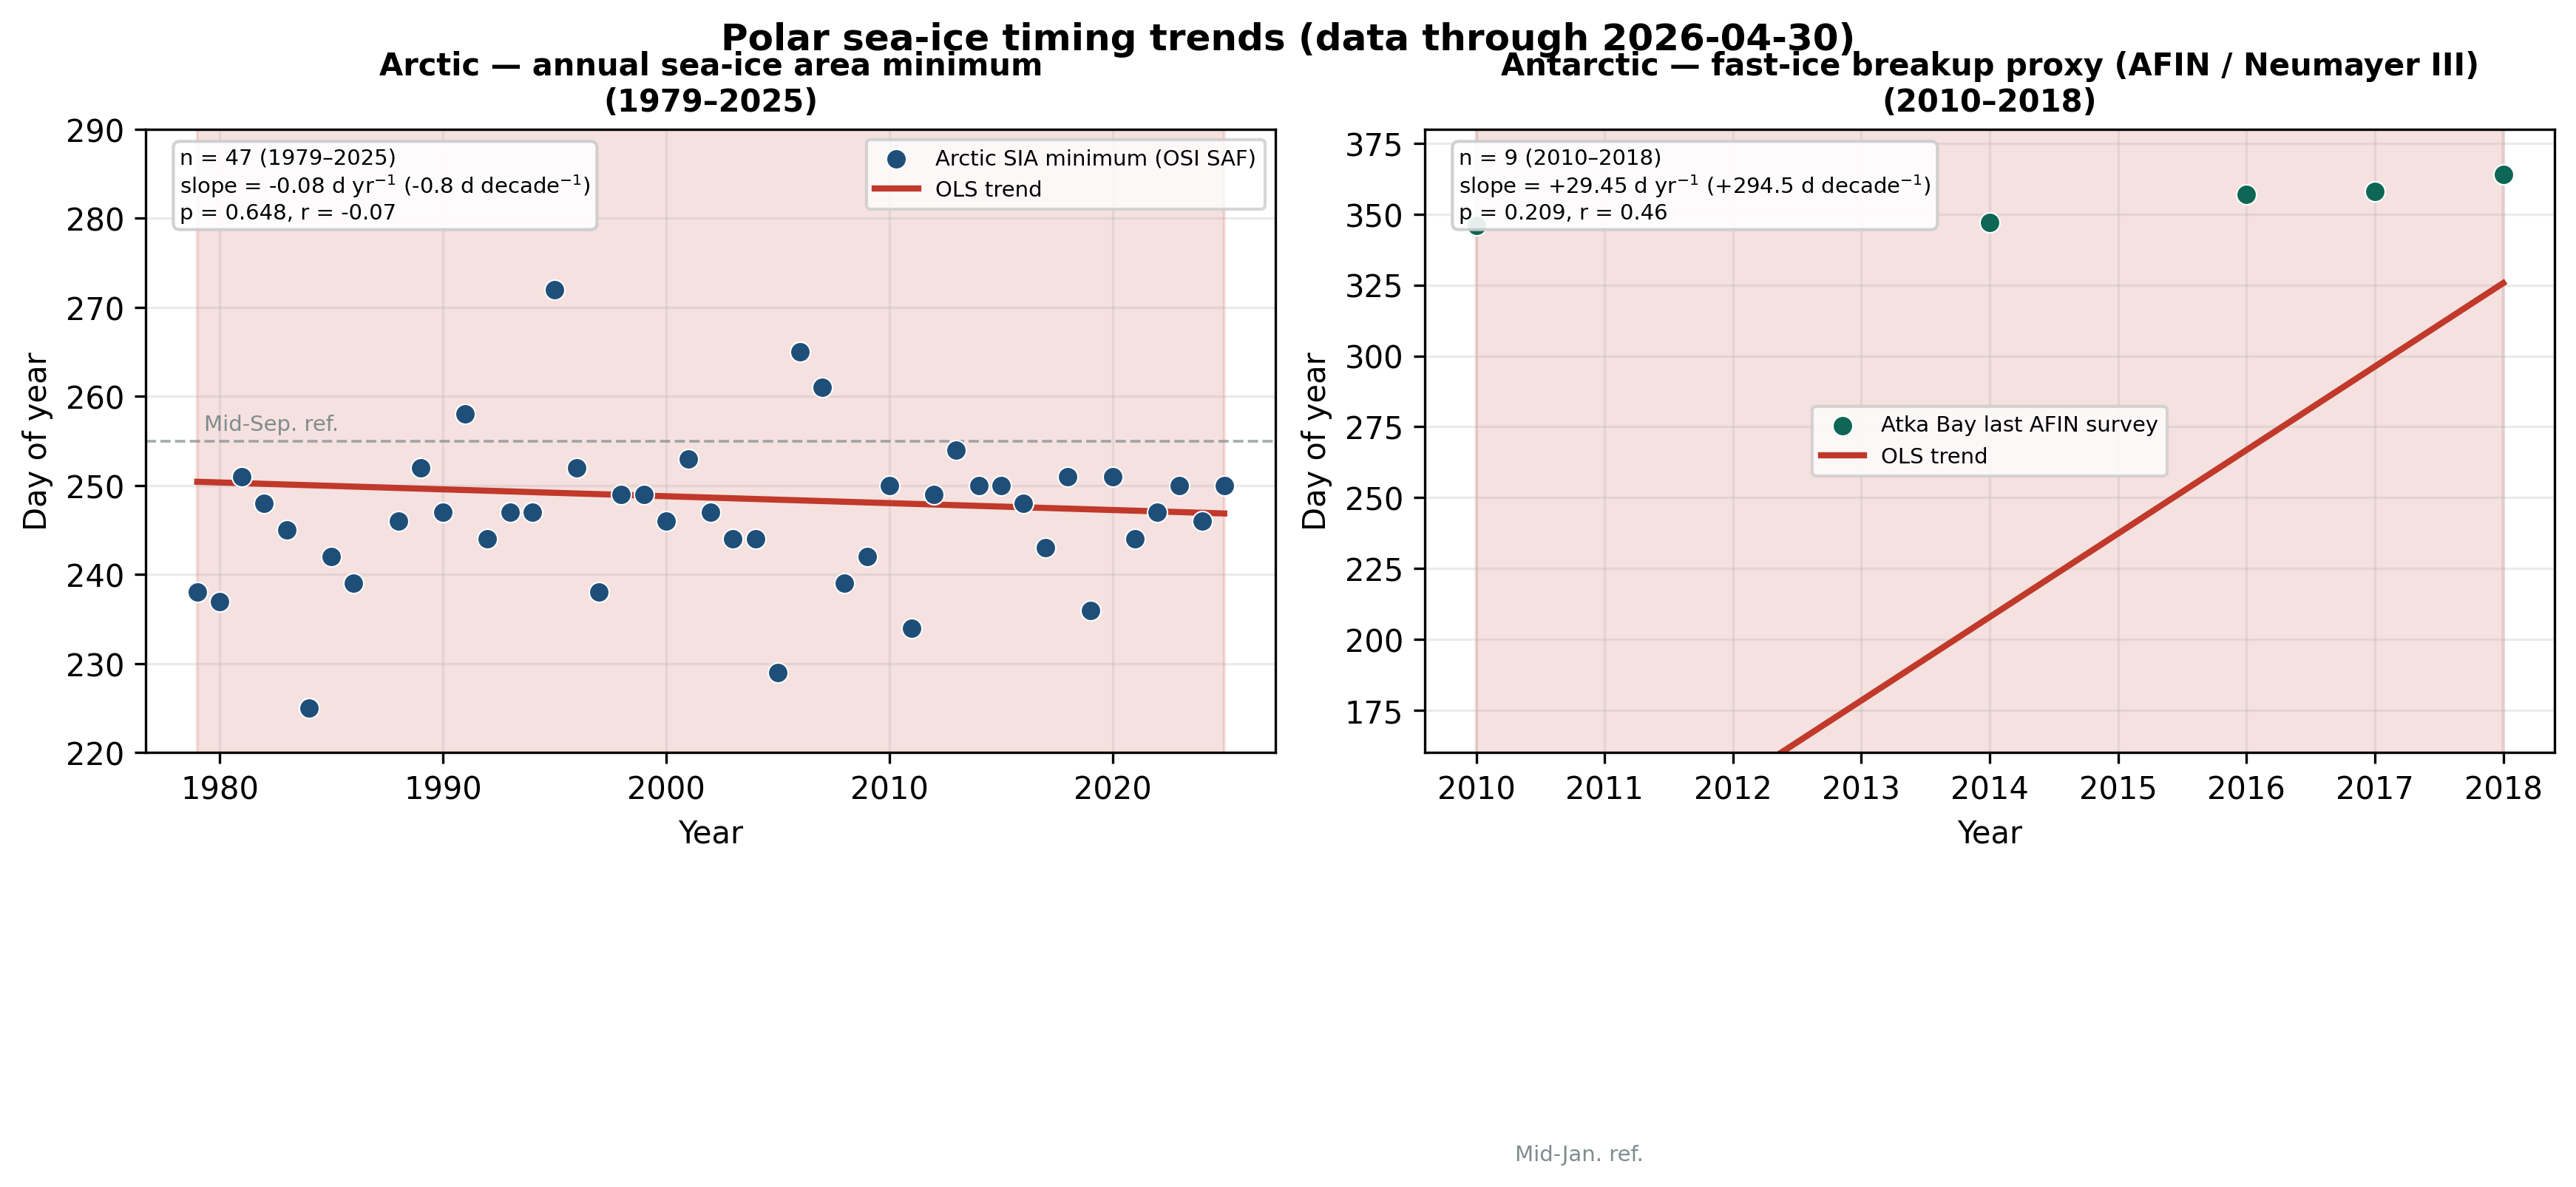
\includegraphics[width=0.92\linewidth]{../results/figures/polar_ice_timing_comparison.png}
\end{frame}

\begin{frame}{Amount $\neq$ timing}
  \centering
  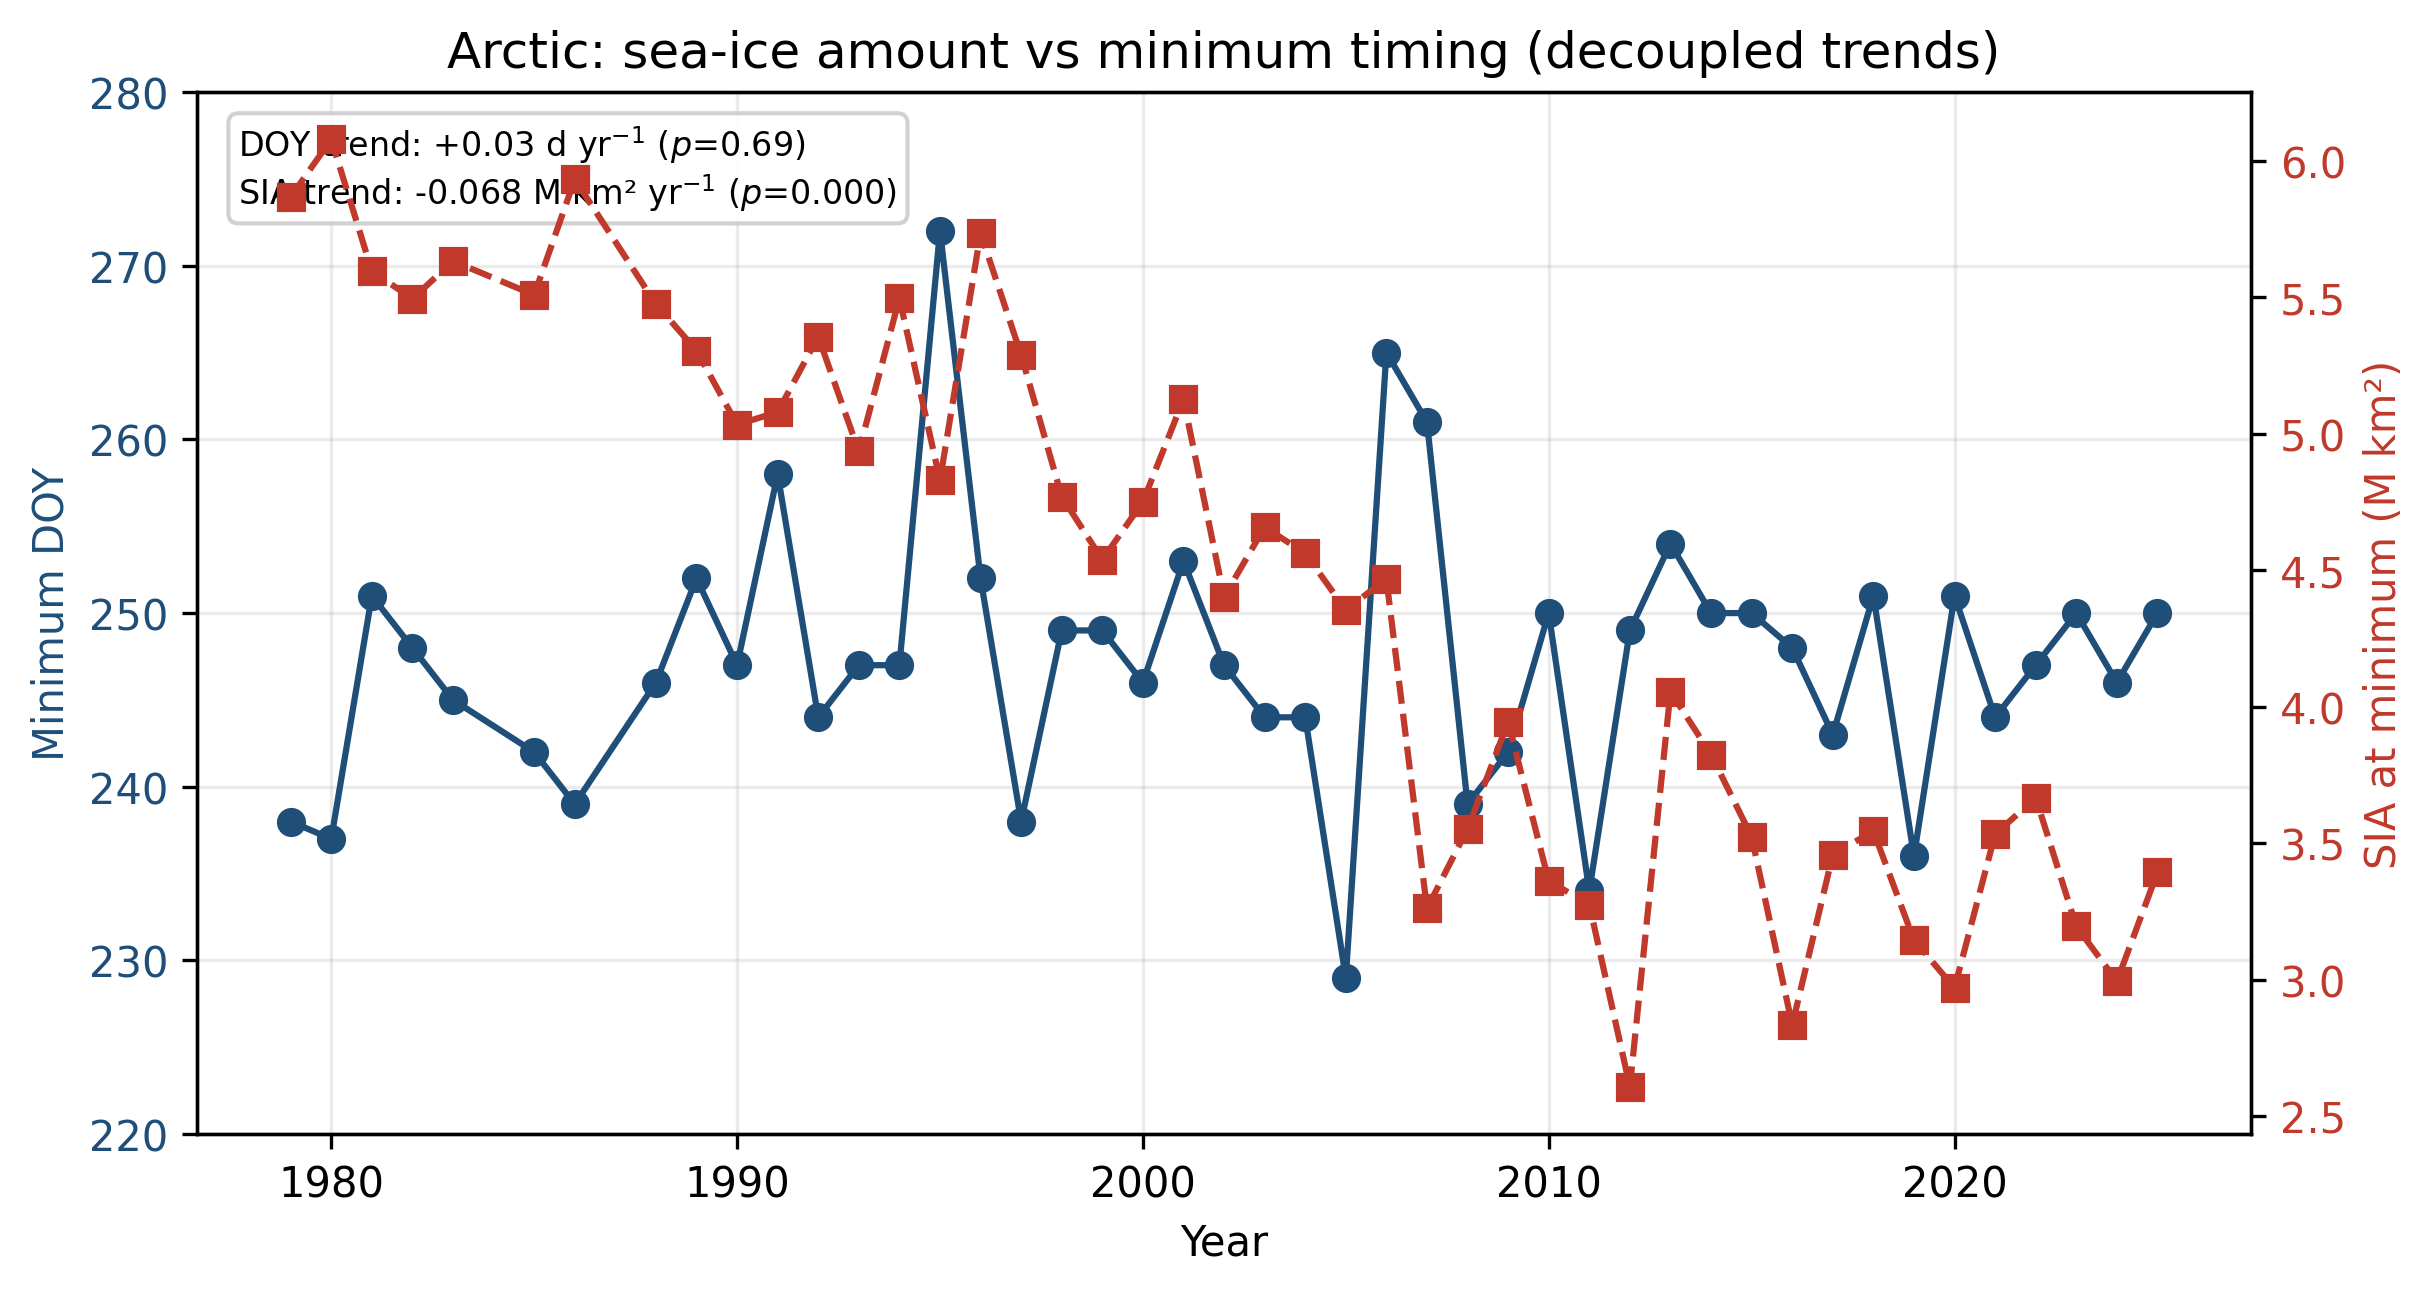
\includegraphics[width=0.88\linewidth]{../results/figures/arctic_sia_minimum_vs_doy_dual_axis.png}
  \vspace{0.3em}
  {\small SIA at minimum declines; minimum \emph{date} does not show a robust trend.}
\end{frame}

\begin{frame}{Phase 2: spatial hypothesis, tested rigorously}
  \centering
  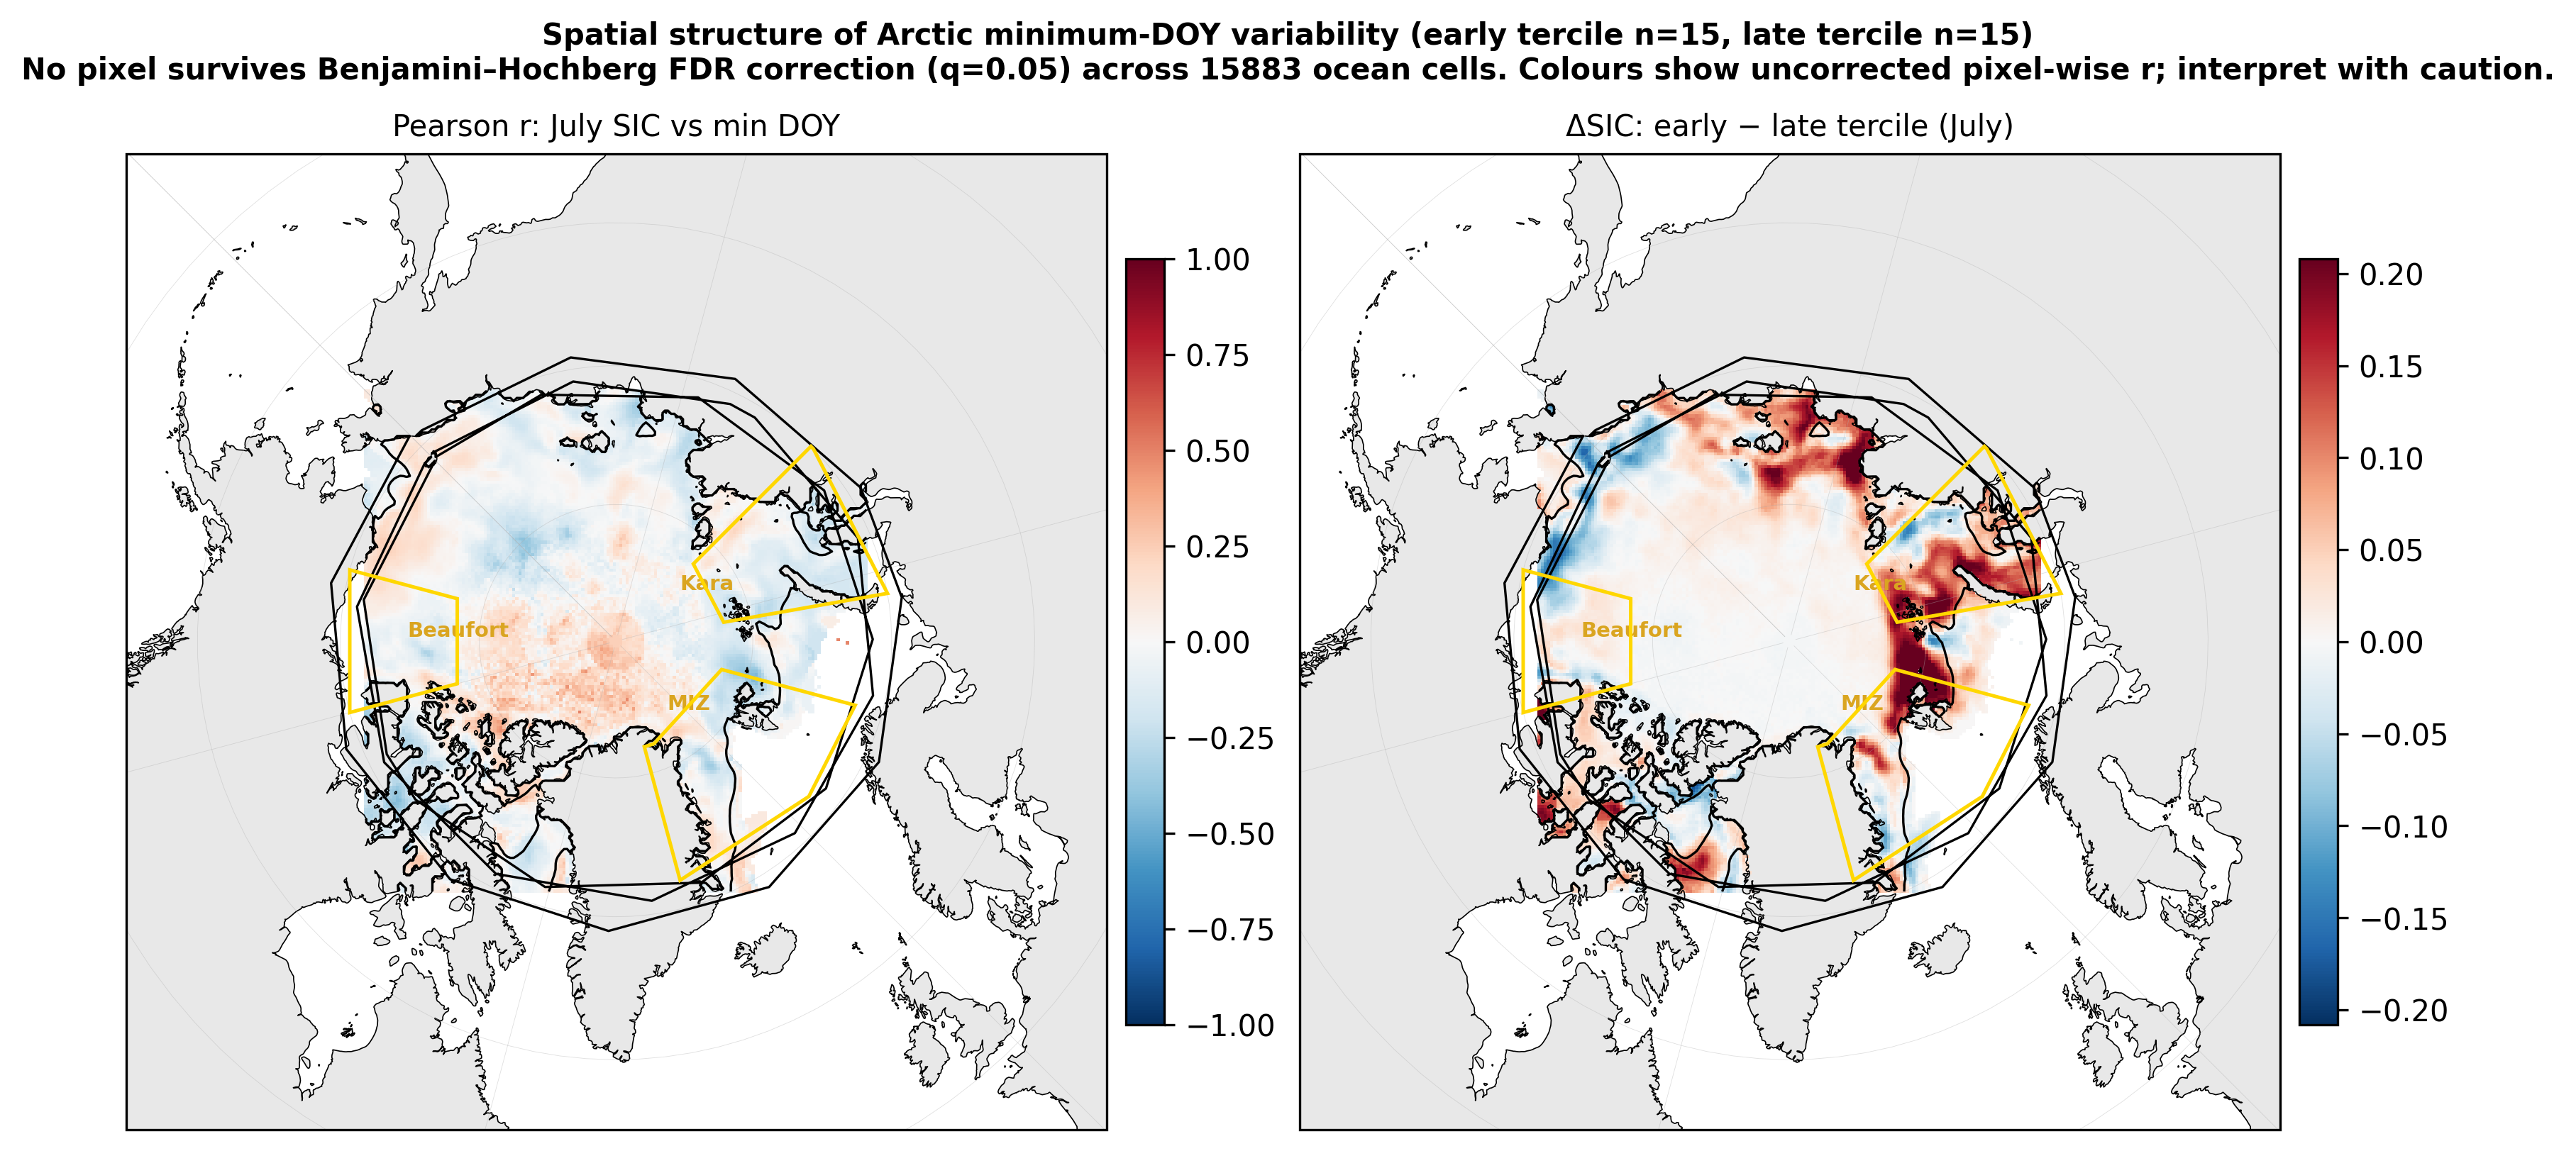
\includegraphics[width=0.92\linewidth]{../results/figures/fig5_spatial_heatmap.png}
  \vspace{0.2em}
  {\small 15{,}883 pixel tests $\rightarrow$ 0 survive FDR correction ($q=0.05$). Beaufort/Kara/MIZ region-mean tests: $p=0.96/0.45/0.39$.}
\end{frame}

\begin{frame}{Why the null result matters}
  \begin{itemize}
    \item An uncorrected correlation map over $\sim$16k pixels \emph{always} shows plausible-looking ``hot spots'' --- that's multiple comparisons, not signal
    \item Static pre-melt (July) SIC does not predict the September minimum date
    \item Literature: timing is driven by \emph{within-season wind forcing} instead --- Beaufort High bursts (Nie et al.\ 2025), easterly-wind ice transport in Kara (Yang et al.\ 2024)
    \item MIZ SIC is itself increasingly noisy day-to-day (+11.4\% since 2007, Wang et al.\ 2026, \textit{GRL}) --- consistent with, not contradicting, our null result
  \end{itemize}
\end{frame}

\begin{frame}{Antarctic context}
  \centering
  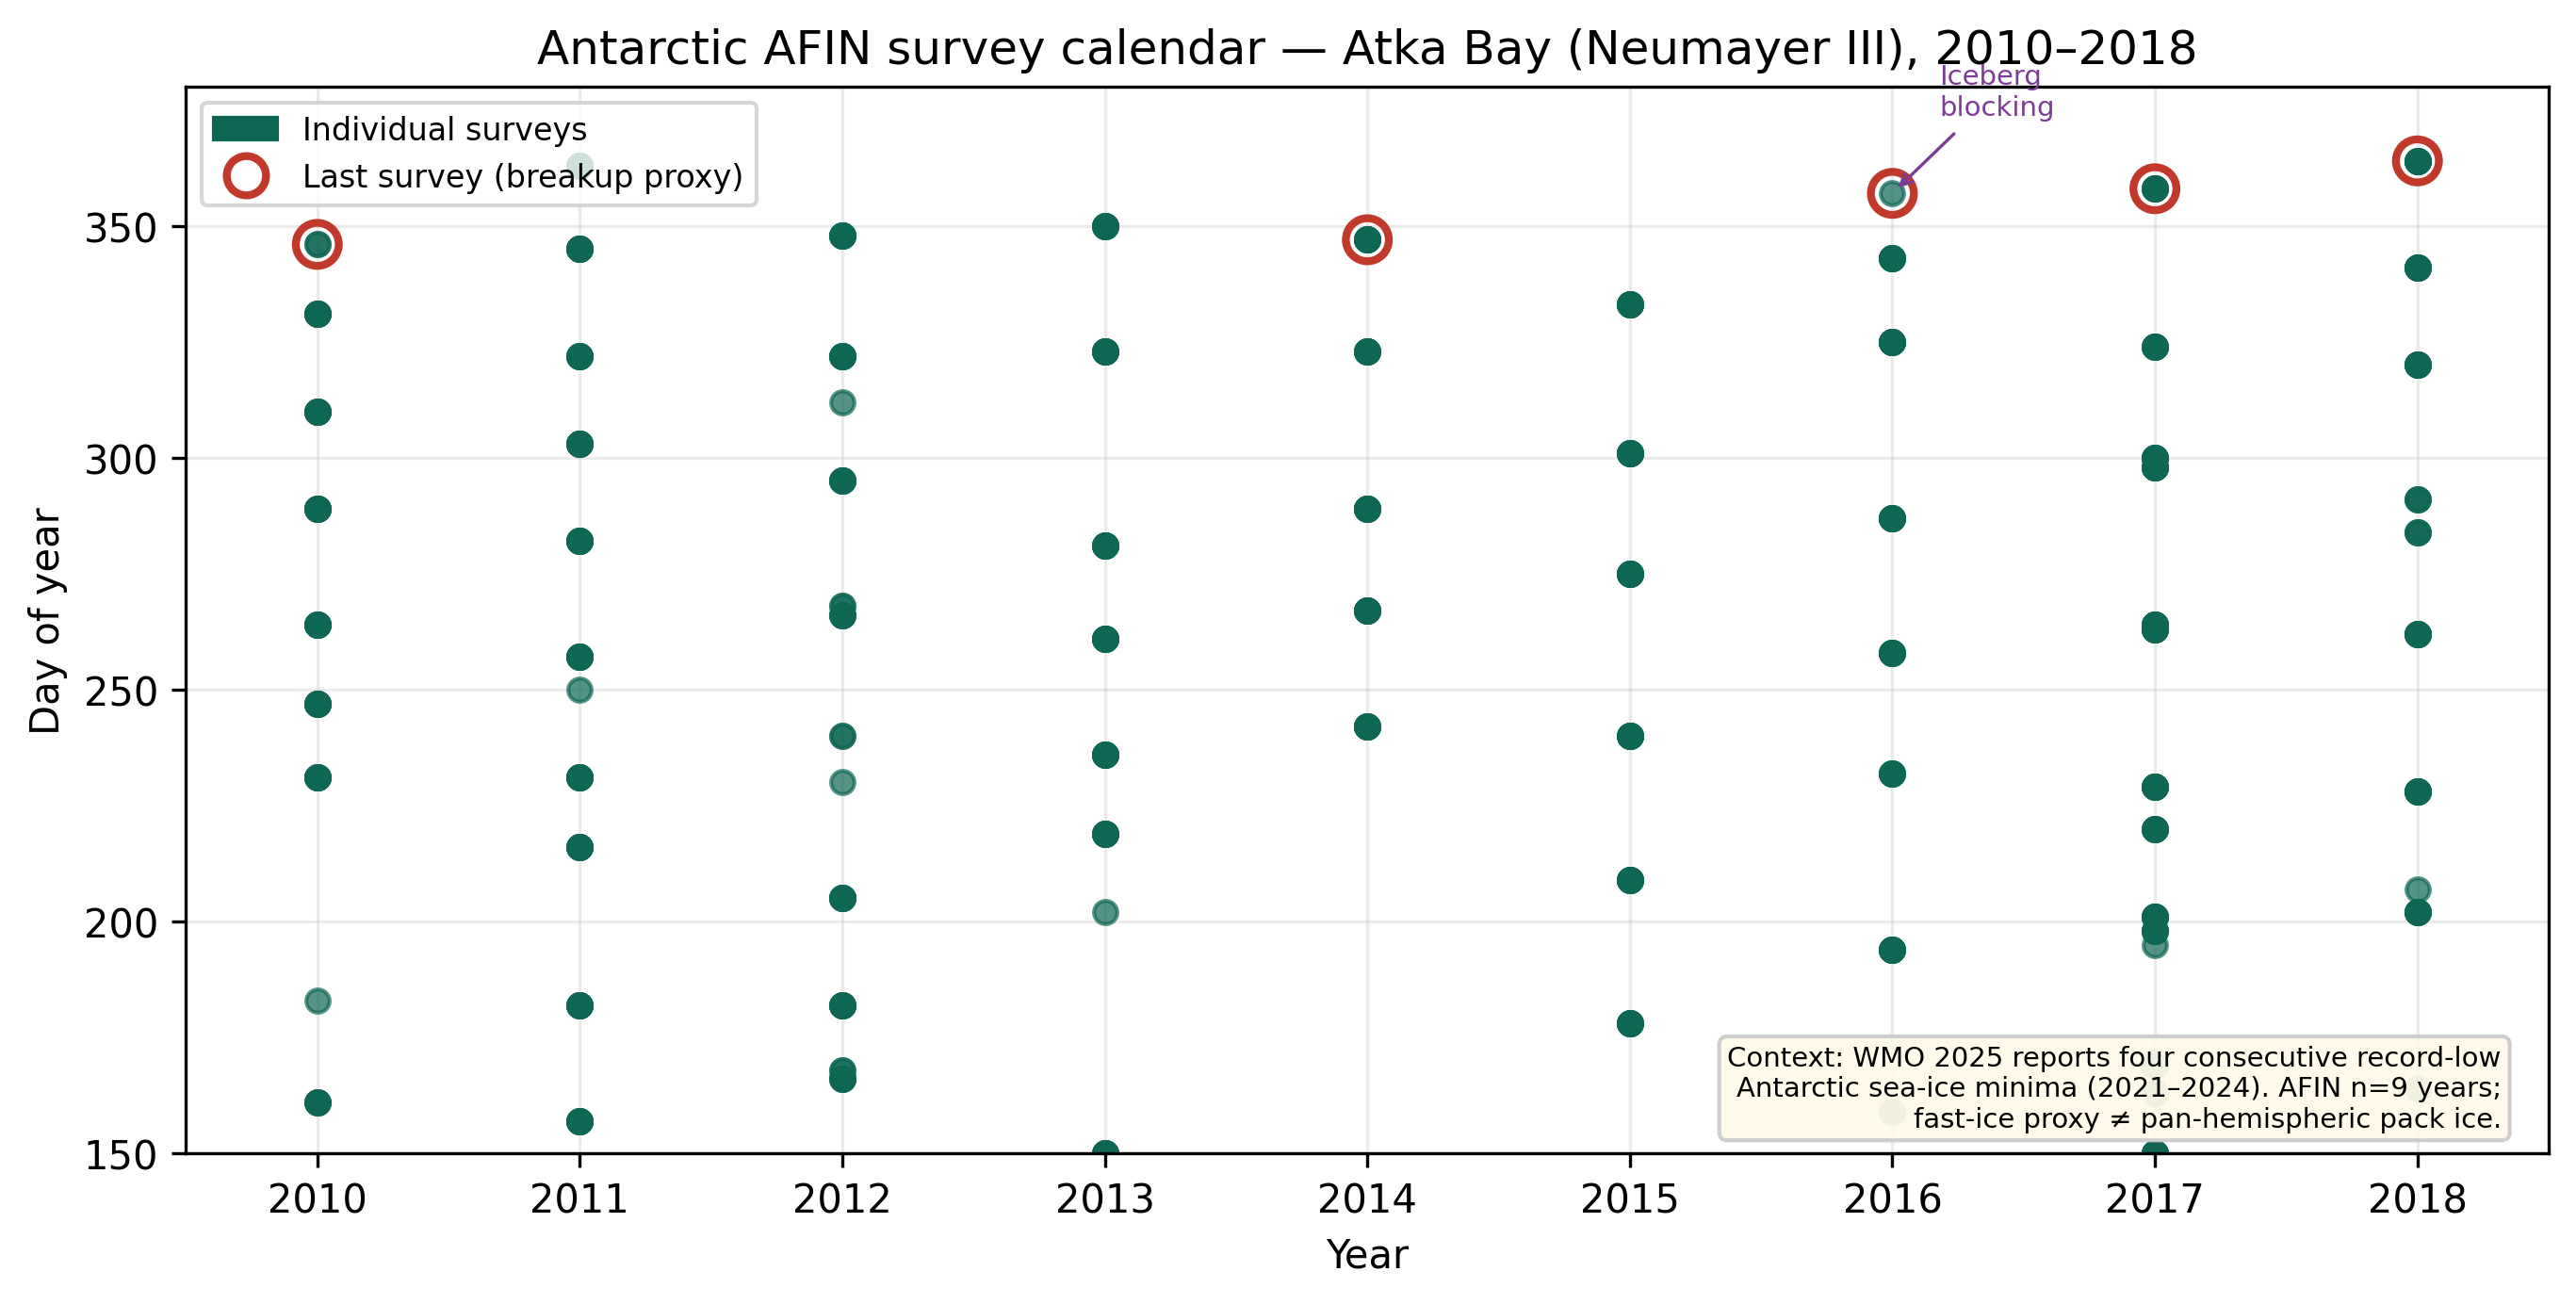
\includegraphics[width=0.88\linewidth]{../results/figures/antarctic_afin_calendar.png}
  \vspace{0.3em}
  {\small AFIN $n=9$; WMO~(2026): four lowest Antarctic sea-ice minima on record, 2022--2025.}
\end{frame}

\begin{frame}{Conclusion}
  \begin{quote}
    Pan-hemispheric timing shows no significant trend. Naive spatial preconditioning doesn't explain the variability either --- both point to internal, weather-driven noise rather than a learnable geographic fingerprint.
  \end{quote}
  \textbf{Next step (future work):} correlate minimum DOY with ERA5 wind fields, not static SIC.
\end{frame}

\end{document}
